\documentclass[a4paper]{article}

\usepackage{hyperref}
\usepackage{circuitikz}
\usepackage{amsmath}
\usepackage{amsfonts}
\usepackage{mathtools}
\usepackage{physics}

\usepackage{import}
\usepackage{xifthen}
\usepackage{pdfpages}
\usepackage{transparent}

\newcommand{\incfig}[1]{
    \def\svgwidth{\columnwidth}
    \import{./figures/}{#1.pdf_tex}
}

\title{FP09 - Neuromorphic computing}
\author{R. Dorstijn (sd249) \& Moritz Epping (hh234)}
\date{December 2020}

\begin{document}
\maketitle

\section{Introduction}
\subsection{General theoretical background}
\subsubsection{Motivation}
Brains and computers often are compared because of their shared purpose,
decision making, though they have irreconcilable differences in architecture.
Modern computers function on the basis of the van Neumann
architecture\cite{von-Neumann}, which separates the control unit from the memory
and the computation unit. Though it simplifies the structure of the computer and
makes it modular, it does create a clear bottleneck at the communication layer,
commonly known as the von Neumann bottleneck. This creates an energy
inefficiency that is absolutely unacceptable for biological systems like that of
humans, who spend around 20\% of its total energy uptake on the brain\cite{metabolic-rates}.
This most likely has provided significant evolutionary pressure for hominids to
optimize metabolic resource usage\cite{seymour2016fossil}. For this reason a new
architecture for computers has been suggested: neuromorphic\footnote{``Neuro''
as in brain, ``-morphic'' as in having the shape of, forming ``having the shape
of a brain''.} computing.

\subsubsection{Signal processing in the brain}
Neurons (see fig \ref{fig:neuron}) are the basic computational components of the
brain, transmitting and morphing signals. Each neuron receives signals from
others at the dendrites, which shift the electric potential at the membrane of
the cell at the site of the synapse\footnote{The connection point of two
dendrites where the axon of one meets the dendrite of the other.}, creating an
ion wave crossing the entire membrane of the neuron, reaching it's axon,
allowing it to pass the signal on to other neurons.

\begin{figure}
    \centering
    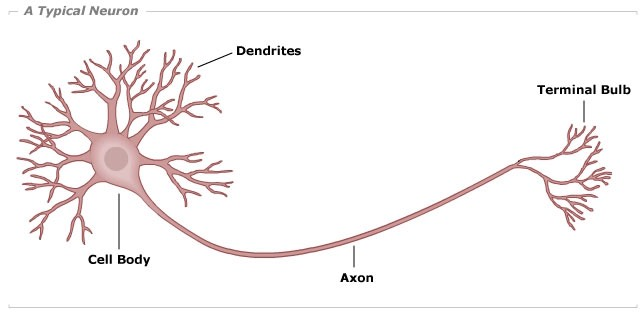
\includegraphics[width=\textwidth]{figures/neuron.jpg}
    \caption{Schematic image of a neuron, showing the dendrites, soma and axon.
    Source: Pennsylvania State University}
    \label{fig:neuron}
\end{figure}

The potential at the neuron membrane as a function of time is plotted in figure
\ref{fig:action-potential}, here it is demonstrated how a potential shift caused
by pre-synaptic\footnote{That is the neuron that passes on a signal to the
post-synaptic one.} neurons initiates a spike in the membrane potential, which
forces a release of ion containing vesicles at the terminal bulb, facilitating
the transfer of the signal by changing the relative potential at the dendrites.

\begin{figure}
    \centering
    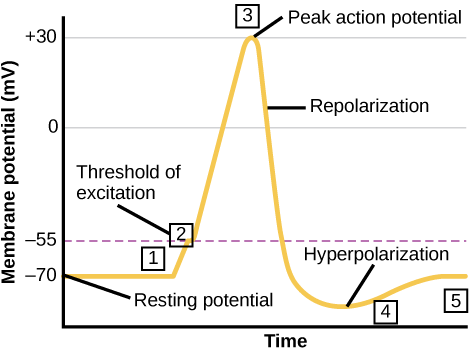
\includegraphics[width=.6\textwidth]{figures/action-potential.png}
    \caption{Formation of an action potential. Source: \\ \url{https://courses.lumenlearning.com/boundless-biology/chapter/how-neurons-communicate/}}
    \label{fig:action-potential}
\end{figure}

In order to emulate the behaviour electronically, a leaky integrate and fire
(LIF) model is used. A single neuron is represented by an electronic circuit
like the one in figure \ref{fig:circuit}.

\begin{figure}
    \centering
    \begin{circuitikz}
        \draw (0, 0)    to node[midway, above]{$V_m$} (8, 0) node[op amp, anchor=+](A1){}; % main line
        \draw (A1.out)  to[short, l=$V_\text{out}$, -o] ++(1, 0);
        \draw (7, 1)    node[left, above] {$V_\text{thres}$} to[short, *-] (A1.-);
        \draw (0, 0)    to[vR, l=$g_l$, *-] (0, -2)
                        to[battery1, l=$E_l$] (0, -3) node[ground] {} (0, -4);
        \draw (2, 0)    to[vR, l=$g_x$, *-] (2, -2)
                        to[battery1, l=$E_x$] (2, -3) node[ground] {} (2, -4);
        \draw (4, 0)    to[vR, l=$g_i$, *-] (4, -2)
                        to[battery1, l=$E_g$] (4, -3) node[ground] {} (4, -4);
        \draw (6, 0)    to[C, l=$C_m$] (6, -2)
                        node[ground] {} (6, -2);
        \draw (8, -3)   to[short, l_=$V_\text{reset}$, o-] (8, -1)
                        to[normal open switch, -*] (8, 0);
    \end{circuitikz}
    \caption{Circuit of a single neuron in a LIF chip.}
    \label{fig:circuit}
\end{figure}


\subsection{Background for the experiments}
\subsubsection{Investigation of a single neuron}
\subsubsection{Calibrating neuron parameters}
% So on for all experiments

\section{Execution \& Results}

\subsection{Investigation of a single neuron}
% Moritz does this part
\subsubsection{Setup/Settings}
\subsubsection{Results}

\subsection{Calibrating neuron parameters}
% Robin does this
\subsubsection{Setup/Settings}
\subsubsection{Results}

\bibliography{main}
\bibliographystyle{ieeetr}

\section{Appendix}
% Notebook PDFs here

\end{document}
